\documentclass[12pt]{report}
\usepackage{float}
\usepackage{pdfpages}
\usepackage{amsmath}
\usepackage{times}
\usepackage{mathptmx}
\usepackage{CJKutf8}
\usepackage{setspace}
%\usepackage{pinyin}

%==
\usepackage[english]{babel}
\usepackage{amssymb,amsfonts,amsmath,amsthm}
\usepackage{graphicx}
\usepackage{makeidx}
\usepackage{hyperref}
\usepackage[toc,page]{appendix}
%==
\usepackage[a4paper,left=3cm,top=3cm,right=3cm,bottom=3cm,nohead]{geometry}

\usepackage{algorithm}
\usepackage{enumerate}
\usepackage{algpseudocode}

%
% ---- probabilities ----

% ---- others ----
\newtheorem{theorem}{Theorem}[section]
\newtheorem{corollary}{Corollary}[theorem]
\newtheorem{lemma}[theorem]{Lemma}
\doublespacing
\pagestyle{plain}

\begin{document}
\onehalfspacing

%\renewcommand{\baselinestretch}{1.5} 

\begin{titlepage}
\begin{center}

\begin{CJK}{UTF8}{bkai}
\Large{{國立臺灣大學理學院應用數學科學研究所\\碩士論文}}\\
\large{{Institute of Applied Mathematical Science}}\\
\large{College of Science}\\
\Large{{National Taiwan University}}\\
\Large{{Master Thesis}}\\

\hspace*{1cm}~\\
\hspace*{1cm}~\\

\Large{遷移學習應用於\\
二維胰臟影像小區塊方式之腫瘤辨識\\
Applying Transfer Learning on 
2D Patch-Based \\Healthy Pancreas and Pancreatic Tumor Classification}\\

\hspace*{1cm}~\\
\hspace*{1cm}~\\

\Large{楊宛芸\\Wanyun Yang}\\
\hspace*{1cm}~\\
\hspace*{1cm}~\\

\Large{指導教授:王偉仲 教授\\Wei-Chung Wang, Ph.D.}\\
\hspace*{1cm}~\\
\hspace*{1cm}~\\

%看要不要"日"
\Large{中華民國 109 年 8 月}\\ 
\Large{August, 2020}\\ 
%February, 2020}\\
%\today

\end{CJK}
\end{center}
\end{titlepage}

\pagenumbering{roman}
\setcounter{page}{1}


\addcontentsline{toc}{chapter}{口試委員會審定書}
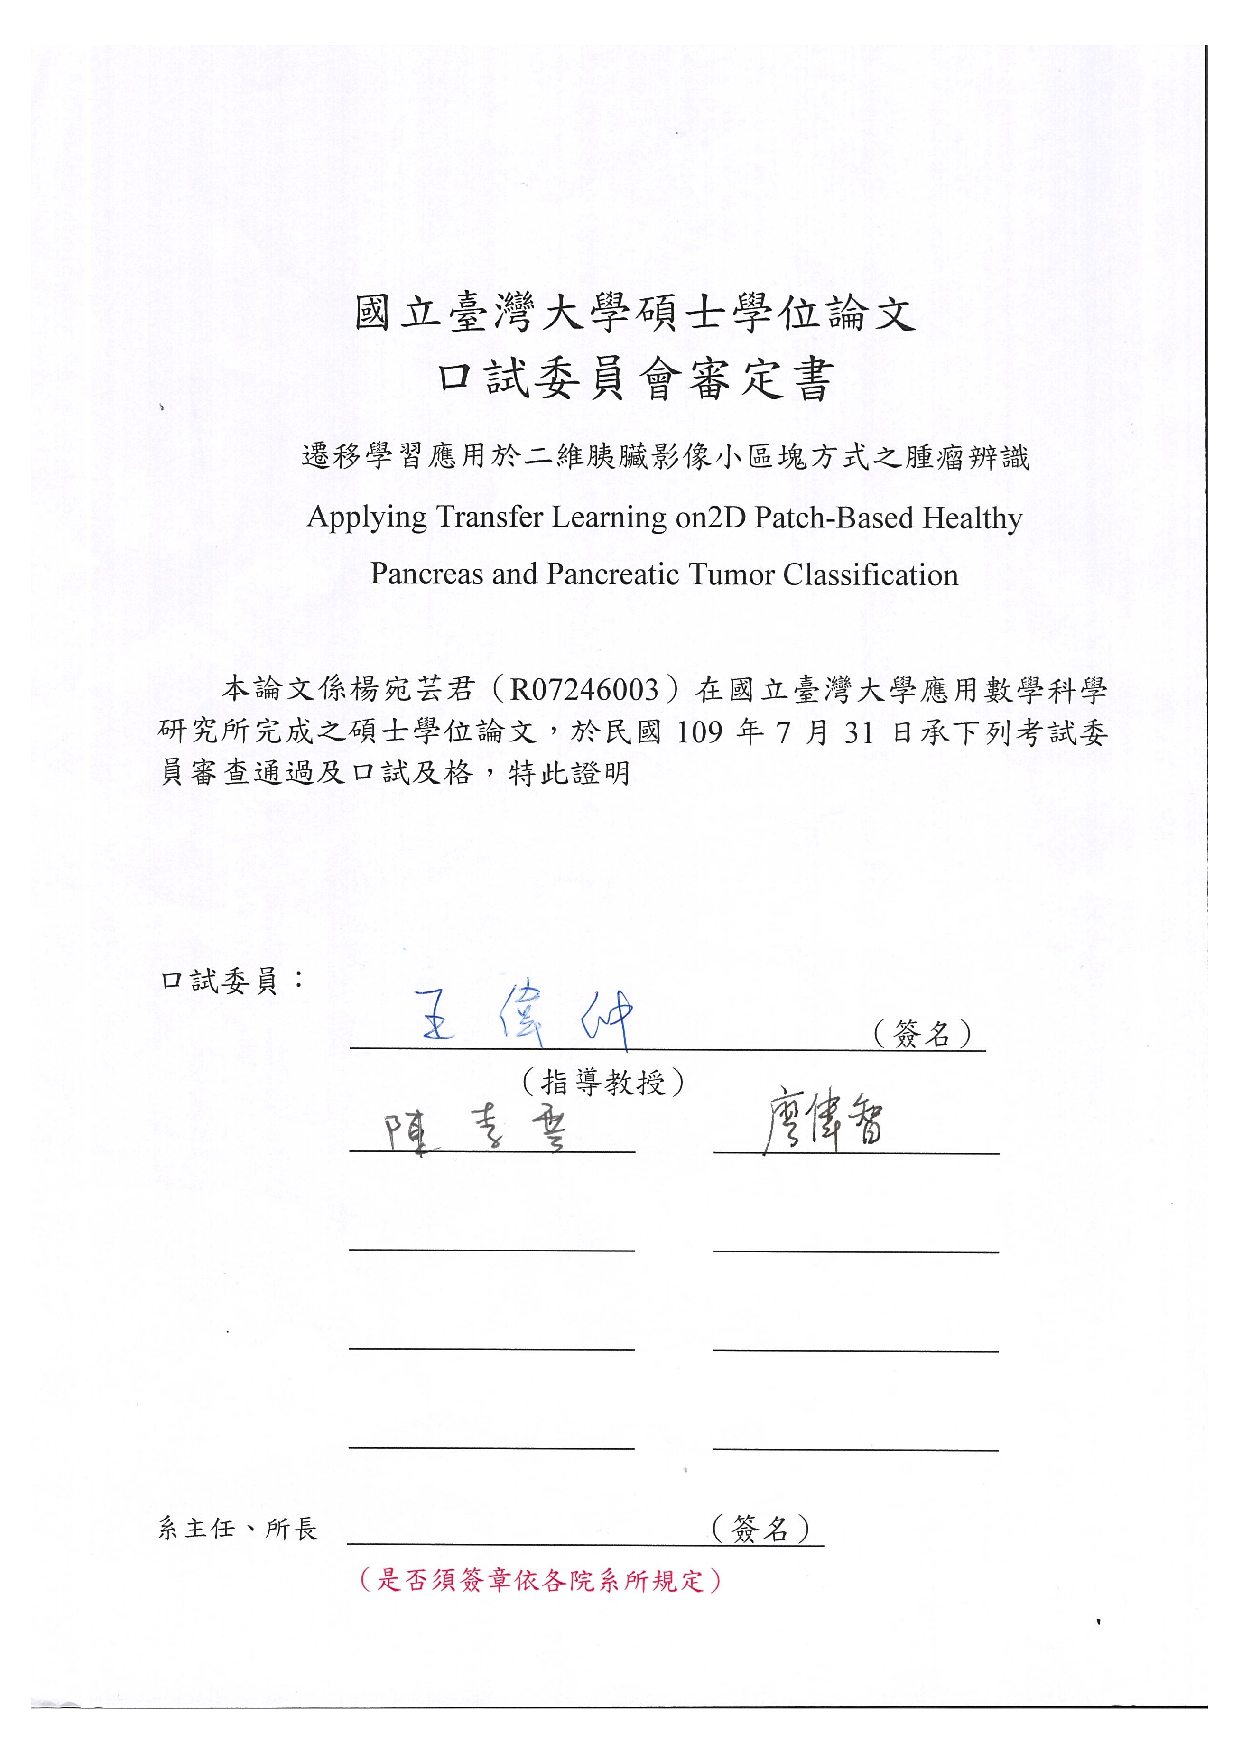
\includepdf[pages=1,pagecommand={},width=\textwidth]{doc.pdf}


%\usepackage[a4paper,left=3cm,top=3cm,right=3cm,bottom=2cm,nohead]{geometry}

\doublespacing

\begin{center}
\Large{{Acknowledgement}}\\
\end{center}
I would first like to thank my thesis advisor, professor Weichung Wang. His lab provides rich learning resources and precious opportunities. He consistently allowed this paper to be my own work, but steered me in the right the direction whenever I have difficulties in research. 

I would also like to thank the doctors at National Taiwan University Hospital who were involved in the pancreatic project: Dr. Wei-Chih Liao and Dr. Poting Chen. Without their medical professionalism and advice on research method, the research could not have been successfully conducted. 

I'm glad to thank a excellent research assistant Tinghui Wu of the Academia Sinica as the second reader of this thesis, and I am gratefully indebted to her for her very valuable comments on this thesis. She also kindly helped me for both programming and experiment setting. 

Finally, I must express my very profound gratitude to my parents and to my friends Chunshuo Chen and YuYuan Yuan. At the end of the second semester of master degree, I was stranded at a bottleneck of my research. They provided me with practical support and encouragement throughout my dilemma and through the process of researching and writing this thesis.  This accomplishment would not have been possible without them. Thank you. 

\clearpage

%\doublespacing

\linespread{1.25}
\begin{CJK}{UTF8}{bkai}

\addcontentsline{toc}{chapter}{摘要}
\begin{center}
\Large{{摘要}}\\
\end{center}
胰腺癌是消化系統中第二常見的癌症,人工智能通常用於協助醫生進行腫瘤檢測。由於包括胰腺在內的所有醫學圖像都是珍貴且難以獲得的,因此我嘗試對圖像進行轉移學習以提高外部數據集的性能。在醫生的幫助下,我獲得了足夠的數據來訓練準確的卷積神經網絡作為基礎分類模型。在此模型的基礎下,我需要將模型使用於不同的數據集,但是在其他數據集上進行測試時,分類模型的性能會降低。我的目標是使用遷移學習方法基於基礎分類模型創造能在外部數據集有精確結果的模型。 \\

在本文中,我們試圖在醫學圖像分析的背景下回答以下核心問題:微調,一種常見的遷移學習方法,如何提高外部數據集的性能;為了獲得一定的性能,我們需要多少數據。我們的實驗一致表明,隨著我們獲得越來越多的外部數據,我們可以獲得對於外部數據更好的預測結果。本文可以幫助評估獲得滿意預測表現所需的外部資料量,並在全球範圍內推廣先前開發的神經網絡模型。此外,還使用增量學習來評估哪個外部掃描圖像(無手動標記)最能改善性能,以便我們可以選擇有價值的數據進行標記。\\

在本文中,我發現混合數據方法和微調方法可以顯著提高外部數據的模型性能。以微調方法為基礎的增量選擇方法可以稍微改善模型性能,但總體而言,它的性能並不比基本的微調更好。\\

關鍵詞:醫療影像、人工智慧、類神經網路、深度學習、遷移學習
\end{CJK}
\doublespacing

\clearpage


%\usepackage[a4paper,left=3cm,top=3cm,right=3cm,bottom=2cm,nohead]{geometry}

\doublespacing
\addcontentsline{toc}{chapter}{Abstract}
\begin{center}
\Large{{Abstract}}\\
\end{center}
Pancreatic cancer is the second most frequent cancer of the digestive system, and artificial intelligence is frequently applied to help doctors with tumor detection. \\

Since all medical images, including pancreas CT, are precious and hard to get, I tried transfer learning on images to improve performance on external dataset. With the help of doctors, I get enough data to train an accurate convolution neural network as source model. In the future I will apply recent model to different datasets, but the AUC performance of classification model decreases when testing on other datasets. My goal is to enhance the performance of model on other dataset. \\

In this paper, I seek to answer the following core question in the context of medical image analysis: how fine-tuning improves the performance on external dataset; how much data we need to get a certain performance. Our experiments consistently demonstrated that, as we get more and more external data, we can get a better prediction result on external data. This paper can help to evaluate how many external data we need to get a satisfying result and help to promote the previous neural network model worldwide. Also, incremental learning was used to evaluate which external scan image (without a manual label) improved the performance most so that we can choose valuable data to label. \\

In this thesis, I found that mixed data method and fine-tuning method can obviously enhance the model performance on external data. The selection method incremental provided can slightly improve the model performance, but overall it doesn't perform better than basic fine-tuning. \\

Key words : Medical Images, Artificial Intelligence, Neural Network, Deep Learning, Transfer Learning


\clearpage
\begin{CJK}{UTF8}{bkai}
\tableofcontents
\listoffigures
\listoftables
\end{CJK}
%%\listoftables
%%\listoffigures
%%\listofalgorithms

\clearpage

\doublespacing
\pagenumbering{arabic}
\setcounter{page}{1}
\setcounter{tocdepth}{1}


\chapter{Introduction}
\section{Background}
\subsection{Technical background} 
The medical imaging field has witnessed a new generation of computer-aided systems that show incredible performance with the revival of neural networks owing to the development of parallel computing technique. A Survey on Deep Learning in Medical Image Analysis \cite{litjens2017survey} surveyed the use of deep learning techniques such as image classification, object detection, segmentation, registration.

\subsection{Clinical background}
Pancreatic cancer is a frequent cancer, but it's hard to process. Therefore few theses discussed about this cancer. Pancreatic cancer is the second most frequent cancer of the digestive system which caused 45,750 deaths in the United States in 2019 \cite{siegel2019cancer}. Pancreatic cancer is hard to process because the pancreas’ shape, size and location in the abdomen can vary seriously among patients. These factors make the model less accurate and robust. \cite{Roth2015-mi} 

\subsection{Transfer Learning and Fine-Tuning}
After developing a workable pancreatic neural network model on NTUH dataset, I use fine-tuning, a kind of transfer learning technique, to create another model on a smaller external dataset. There are a sufficiently large pancreatic dataset and a small external pancreatic dataset. Large dataset is applied to help train models for the external pancreatic dataset. Fine-tuning method is used because of this thesis Learning without Forgetting \cite{li2017learning}. The authors compare four methods, including joint training, feature extraction, learning without forget-ting and fine-tuning.  The fine-tuning method performs well in external data, and also has excellent testing efficiency.  Also a thesis in 2017 applies fine-tuning on ultrasound images and has an obvious enhance on model performance. \cite{pan2009survey}

\subsection{incremental Learning}
When training fine-tuning model using unlabeled target data, we need to select unlabeled patient data that provides information most and label them. incremental learning is applied to select patient data that provides most information. AIFT method is applied to do data selection in thesis \cite{zhou2017fine}. It chooses the data that has the highest information entropy and diversity. Fine-tuning model and data selection are applied on pancreatic images in this thesis.



\subsection{Research Team Background}
\cite{liu2020deep} had developed 2D patch-based tumor classification model and want to improve the model performance on external dataset. Our research team started working on pancreatic cancer since 2018 and had developed 2D patch-based tumor classification model based on patient data from National Taiwan University Hospital (NTUH). But when we tested our model using data from other data sources, the performance of the classification model is worse than the previous results. (In this thesis, we mainly use the area under receiver operating characteristic curve (AUC) to evaluate the performance.) Our goal is to improve the performance of model working on external data using fine-tuning technique so that we can apply our model to patient data from different datasets and different countries in the future.

\section{Study objectives}

Consider a source dataset (S) with $ n_S $  patients and an target dataset (T) with $  n_T  $ patients. $  n_S > n_T $. A model trained using source dataset is called source model. Our goal is 
\begin{itemize}
    \item Use source data and target data to build a model that has high AUC performance on target test set.
    \item Evaluate how much target data is needed to improve the AUC performance.
    \item Test the selection method in thesis \cite{zhou2017fine} to evaluate how it improves the AUC performance. 
    % 
\end{itemize}

\chapter{Methods}
 
\section{Previous Experiment and Results}
The thesis is based on the study \cite{liu2020deep}. It provided a proof of concept that CNN can accurately distinguish PC on portal venous CT images. The data criteria, source, format, model and a part of training method of this thesis are the same as \cite{liu2020deep}.

But when we apply the pancreatic model on external data, the performance decrease. The thesis focuses on how to improve the model performance using transfer learning method.


\section{Study Design}
\subsection{Study Goal}
Consider a source dataset and an target dataset. Source dataset has sufficient data to train a model, and target dataset doesn't have sufficient data to train a workable model. The purpose of the thesis is
\begin{itemize}
    \item Use source data and target data to build a model that has high performance on target test set.
    \item Evaluate how many patients are needed to improve the performance.
    \item The selection method in thesis \cite{zhou2017fine} selects a set of target data that can help more on fine-tuning model. 
    % 
\end{itemize}


\section{Data}
\subsection{Data Source}
This thesis applies three datasets. All of them are pancreatic CT images.
\begin{itemize}
    \item {\bf National Taiwan University Hospital\cite{liu2020deep} (ntuh, source data)} \\including both healthy (400) and tumor (400) CT scans. 
    \item {\bf Medical Segmentation Decathlon\cite{simpson2019large} (msd, target data)}\\ including only tumor (182) CT scans. 
    \item {\bf The Cancer Imaging Archive\cite{roth} (tcia, target data)}\\ including only healthy (82) CT scans. 
\end{itemize}

\subsection{Data Criteria}
\subsubsection{National Taiwan University Hospital}
CT images with histologically-/cytologically-confirmed pancreatic adenocarcinoma were applied in this study.

After removing patients’ personal identity, all CT images were examined by two radiologists Kao-Lang Liu and Po-Ting Chen. A diagnostic report would be selected if definite description of pancreatic tumor in included. Otherwise the report would be considered as a missed data. 408 PC patients and 471 negative patients diagnosed from January 1, 2006 to December 31, 2018 were applied in this study.

We performed CT examinations using six scanners listed below
\begin{table}[H]
\centering 
\caption{Scanners}

\begin{tabular}{|l|l|l|l|} 
\hline
Machine  & Company & City & Country  \\ 
\hline
Brilliance iCT 256 & Philips Healthcare & Best & Netherlands           \\ 
\hline
Sensation 64 & Siemens Healthcare & Forchheim & Germany              \\ 
\hline
SOMATOM Definition AS+ & Siemens Healthcare & Forchheim & Germany               \\ 
\hline
Aquilion one & Toshiba & Tochigi & Japan              \\
\hline
Revolution CT &  GE Medical system & Milwaukee & US              \\
\hline
LightSpeed VCT & GE Medical system & Milwaukee & US              \\
\hline
\end{tabular}
\end{table}

with 100, 120, 130 kV or automatic mA control without extra noise reduction processes. The slice thicknes s was 0.7 mm to 1.5 mm, and the image size fixed 512 $ \times $ 512 pixels. The portal venous scan was obtained at 70-80 seconds after intravenous administration of contrast medium. The amount of the contrast medium (mL) was calculated by multiplying the body weight (in kilograms) by 1.5, but no more than 150 mL. All images were reconstructed into 5 mm slices for further analysis. \cite{liu2020deep}

In this study, patients or the public were not involved in the design, or conduct, or reporting, or dissemination. 

\subsubsection{Medical Segmentation Decathlon}
Patients undergoing resection of pancreatic masses is in the dataset. Images were from Memorial Sloan Kettering Cancer Center (New York, NY, USA). There were 420 portal venous phase CT scans iin the dataset . The scans were obtained with the following reconstruction and acquisition parameters: automatic tube current modulation range, 220–380 mA; 120 kVp; and axial slices
reconstructed at 2.5 mm intervals. The pancreatic tumor were manually segmented in each slice by an experienced radiologist using the Scout application. \cite{simpson2019large} 


\subsubsection{The Cancer Imaging Archive}
The National Institutes of Health Clinical Center provided 82 abdominal contrast enhanced 3D CT scans from 53 male and 27 female patients. Seventeen of patients are healthy kidney donors scanned prior to nephrectomy. The rest of 65 patients were selected by a radiologist from healthy patients. Patients' ages range from 18 to 76 years. The size of CT scans fixed 512 $\times$ 512 pixels with varying pixel sizes and slice thickness between 1.5 - 2.5 mm. The CT scans were acquired on Philips and Siemens MDCT scanners (120 kVp tube voltage). A medical student manually performed slice-by-slice segmentation of all scans as ground-truth and were verified/modified by an expert radiologist. 
\cite{roth}

\subsection{Data Format}
Each CT scan contained three images: one pancreas image, one non-cancerous pancreatic label and one cancerous pancreatic label. Figure showed one set of images. (add images)



\subsection{Data Partitions}


A window with width 250 Hounsfield unit (HU) and length 75 HU is applied to get 2d square CT images patches. All patches are normalized to [0,1] using linear interpolation and the patches which are neither pancreas nor tumor are excluded. Then move the window with step size half of the patch size to generate overlapped data to increase the variance and size of the dataset. Patches including any pancreatic cancer are defined to be cancerous patches while the rest are defined to be healthy ones.

Two experienced abdominal radiologists Kao-Lang Liu and Po-Ting Chen with at least 5 years of working experience manually labeled all CT images using software (3D slicer version 4.8.1) for further experiments. Since the border between the pancreas and surrounding tissue is not clear, two doctors jointly review all images.

All axial CT images that contained the pancreas or pancreatic cancer were manually labeled for further processing using an open source software (3D Slicer version 4.8.1) by one of two experienced abdominal radiologists (PTC and KLL) with at least 5 years of working experience. Because of the indistinct border of pancreas with the surrounding tissue, all labeled images were jointly reviewed for consensus by the radiologists.
 The window width and window level of all CT scans were 250 Hounsfield unit (HU) and 75 HU, respectively. Linear interpolation was used to normalize all images to [0, 1]. The region that were neither pancreas nor tumor were excluded from images. The images were then cropped into 2D square patches using the moving window method. The moving distance was set as half of the patch dimension to generate overlapping patches in order to increase the variation and size of training data. The patches which contained any pancreatic cancer were defined as cancerous, whereas patches that contained only non-cancerous pancreas were defined as non-cancerous.
 \\
A deep CNN was trained to predict the probability that a patch harbors PC and classify the patch as cancerous or non-cancerous using all patches of the training/validation set. The optimal patch size was determined by comparing the result of models trained with different sizes patches. \cite{liu2020deep}

\section{Model}
The CNN model in this thesis was modified from VGG network which was a widely-used neural network in image classification. Weighted binary cross-entropy was selected as the loss function since the classification problem was imbalanced. Table 1 provides the details of the model, and the layer structures, kernel sizes, channels, and output sizes of the network were included in the table. \cite{liu2020deep}

\begin{table}[H]
\centering
\caption{CNN model Structure}
\begin{tabular}{|l|l|l|} 
\hline
Layer (type)              & Output Shape      & Parameter  \\ 
\hline
conv2d 1 (Conv2D)             & (None, 50, 50, 16) &  416 \\
\hline
conv2d 2 (Conv2D)        & (None, 50, 50, 32)                        & 12832        \\
\hline
max pooling2d 1 (MaxPooling2) &  (None, 50, 50, 32) &  0         \\
\hline
conv2d 3 (Conv2D)                                    & (None, 25, 25, 64)                        & 18496                            \\
\hline
conv2d 4 (Conv2D)             & (None, 25, 25, 64) & 36928     \\
\hline
max pooling2d 2 (MaxPooling2)                        & (None, 12, 12, 64)                        & 0                                \\
\hline
conv2d 5 (Conv2D)                                    & (None, 12, 12, 128)                       & 73856                            \\
\hline
conv2d 6 (Conv2D)                                    & (None, 12, 12, 128)                       & 147584                           \\
\hline
max pooling2d 3 (MaxPooling2)                        & (None, 6, 6, 128)                         & 0                                \\
\hline
flatten 1 (Flatten)                                  & (None, 4608)                              & 0                                \\
\hline
dense 1 (Dense)                                      & (None, 32)                                & 147488                           \\
\hline
dropout 1 (Dropout)                                  & (None, 32)                                & 0                                \\
\hline
dense 2 (Dense)                                      & (None, 32)                                & 1056                             \\
\hline
dense 3 (Dense)                                      & (None, 1)                                 & 33 \\
\hline
\end{tabular}
\end{table}


\section{Training}
Two callbacks were used to monitor the validation loss during the process in order to optimize model performance. 
First, if loss did not decrease within ten iterations, the learning rate would decrease to 10 percent. After that, early stopping callback would break the training process after the validation loss remained stable after 40 iterations to avoid overfitting. Python (version 3.6.8) using Keras (version 2.2.4) and Tensorflow (version 1.7.0) libraries were used to write the codes.

The number of epochs of most experiments is 200, but for incremental learning experiments, the number changes because of different training process. \cite{liu2020deep}


\chapter{Experiments}
There are 8 experiments in this thesis which can be classified into four parts: basic models, mixed data model, fine-tuning models, and increment fine-tuning models. In the first part, I train models in order to compare with other experiments and choose some parameters. In mixed-data part, I try to train models using both source and target data. When it comes to fine-tuning part, I use target data to fine-tune source model. Finally, I try to add target data gradually into fine-tuned model.

\section{Cross Validation}
I use cross validation to validate my model and divide training/validation/testing sets. Cross validation is validation techniques for assessing how the results of a model will generalize to an independent dataset and estimating how accurately a predictive model will perform in practice. I divide dataset into 10 subsets. Then I choose one to be testing set while the rest part is training set and validation set. For the rest 9 subset, I choose 10 \% to be validation set and the rest 90 \% is training set. The two tables below shows how we divide training/validation/testing sets for source data and target data.


\begin{figure}[H]
    \hfil
    \begin{minipage}[t]{0.9\textwidth}
        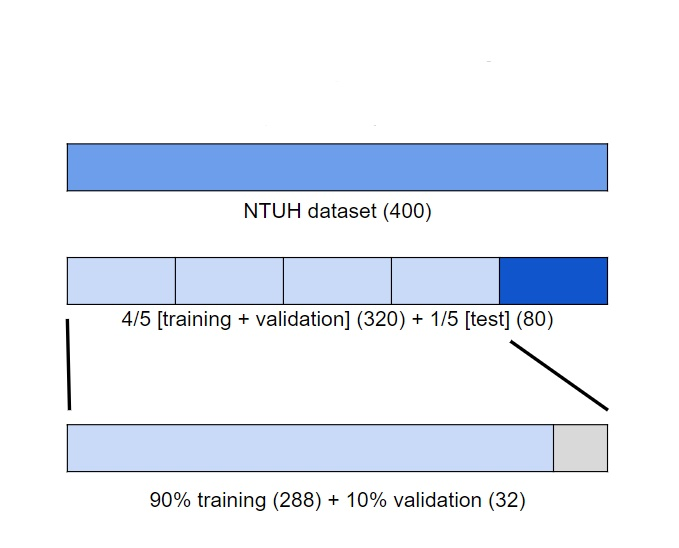
\includegraphics[width=\textwidth]{fig/cross.png}
        \caption{\label{fig:parallel1} AUC for mixed Source Data and Target Data}
    \end{minipage}
    \hfil
\end{figure}
 
 \begin{table}[H]
\centering
\caption{training/validation/testing set (10 folder)}
\begin{tabular}{|l|l|l|l|l|} 
\hline
~            & source H & source T & target H (tcia) & target T (msd)  \\ 
\hline
train        & 330      & 382      & -               & -               \\ 
\hline
validation   & 37       & 42       & -               & -               \\ 
\hline
source test  & 41       & 47       & 0               & 0               \\ 
\hline
target test~ & 0        & 0        & 8               & 18              \\
\hline
\end{tabular}
\end{table}
\begin{table}[H]
\centering 
\caption{training/validation/testing set (B) (10 folder)}
\begin{tabular}{|l|l|l|l|l|} 
\hline
amount of data   & tar H (train) & tar T (train) & tar H (val) & tar T (val)  \\ 
\hline
40       & 11      & 25      & 1               & 3               \\ 
\hline
80 & 22       & 50       & 2               & 6               \\ 
\hline
120 & 34       & 74       & 4               & 8               \\ 
\hline
160 & 45        & 99        & 5               & 11              \\
\hline
200 & 56       & 125       & 6               & 14               \\ 
\hline
\end{tabular}
\end{table}
 ~\\
\section{Basic Models}
In this part, I train models in order to compare with other experiments and choose parameters for other experiments.
\subsection{Train Models Using Only Source Data (B1)}
First, I want to calculate the prediction results if the model is only consider about source data. The results will compare with other experiment results to see how much other methods will improve. The amount of target data fixes 0.
\subsection{Train Models Using Only Target Data (B2)}
I want to calculate the prediction results if the model is only consider about target data. I want to know if how much data is needed to get a sufficiently nice model. The amount of target data varies from 40 to 200.
\subsection{Choose the Number of Fixed Layers in Fine-tuning Experiments (B3)}
All experiments in this thesis use a simplified VGG model for training, however it's better to fix some layers since the target dataset is small for fine-tuning. The goal of this experiment is to find the number of fixed layers in fine-tuning experiments. The amount of target data fixes 200.
~\\
\section{Mixed Data Models}
\subsection{Mixed Data Models (M1)}
In this part, we mixed source and target data to train model. The amount of target data varies from 40 to 200 while the amount of source data fixed.
~\\
\section{Fine-Tuning Models}
\subsection{Fine-Tuning Models (F1)}
In this part, I fine-tuned the model trained in (B1) using target data. I fixed the first three layers in this experiments and use target data to modify the rest layers. The amount of target data varies from 40 to 200.
~\\
\section{Increment Fine-Tuning Models}
Suppose we get an unlabeled target dataset, we want to first label some data that best improve the model performance and use them to fine-tune model. If the AUC performance is not good enough, we need to repeat all steps and fine-tune model using another selected dataset.

\subsection{AIFT Selection Method}
AIFT selection method is applied in increment learning. It calculate the entropy and diversity of the patch-based prediction result of each patient data, and select the data that has the maximum entropy and diversity. For each unlabeled patient data, first I split it into patch-based data. Then use the model generated by source data to predict each patch and get a list of prediction results. Secondly, if the mean value of the list is higher than 0.5, choose the top quarter of list. Otherwise choose the last quarter of list. Then calculate the entropy and diversity of the prediction list. Finally choose a set of patient data that has the highest entropy and diversity and label them. 

\subsection{Fine-tuning Using Selected/Random Target Data (S1/R1)}
This experiment is applied to observe the AUC performance and validate if the selection method AIFT works compared to random selection. We replace the select method to random selection to valid that the selection method really works. 

\subsection{Fine-tuning Using Different Amount of Target data (S2/R2)}
We gradually add selected subset of target data until all target data is used to observe the AUC performance. The amount of target data varies from 40 to 200.

\subsection{Fine-tuning Using Selected/Random Target Data with 66 epochs (S3/R3)}
This experiment is the same as S1/R1 except the number of epochs. I reduce the number of epochs so that the calculation cost is the same as basic fine-tuning method. 
\chapter{Result}
 This chapter consists of two parts: experiment results and comparison. All experiment results are in the first part, and the comparisons of different experiment data are in the second part. To observe the patch-based and patient-based AUC performance on target data, 10-folder cross-validation is applied to validate all the experiments.

\section{Basic Models}
\subsection{Train Models Using Only Source Data (B1)}
This experiment is applied to validate that how much AUC performance other algorithms improve. Only source data is applied for model training. 

Ten-folder cross-validation was performed 3 times to get three sets of source data models. Figure 4.1 and figure 4.2 show the patch-based and patient-based AUC performance of experiment B1, respectively. The patch-based AUC performance on target data varied from 0.71 to 0.84 while the patient-based AUC performance varied from 0.58 to 0.98. The AUC value of source data model will heavily influence the experiment results on transfer learning or incremental learning. \\

\begin{figure}[H]
    \hfil
    \begin{minipage}[t]{0.9\textwidth}
        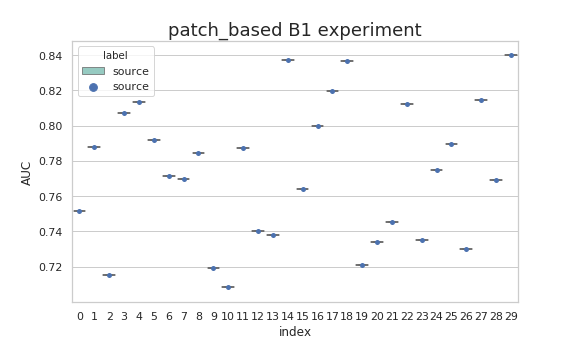
\includegraphics[width=\textwidth]{fig/B1_index_patch.png}
        \caption{\label{fig:parallel1} Patch-based AUC for B1 Experiment (different folder)}
    \end{minipage}
    \hfil
\end{figure}
\begin{figure}[H]
    \hfil
    \begin{minipage}[t]{0.9\textwidth}
        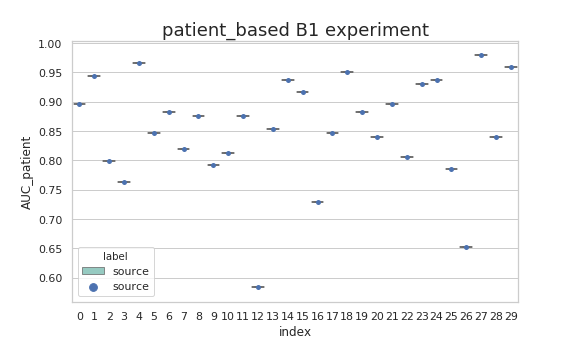
\includegraphics[width=\textwidth]{fig/B1_index_patient.png}
        \caption{\label{fig:parallel1} Patient-based AUC for B1 Experiment (different folder)}
    \end{minipage}
    \hfil
\end{figure}
\subsection{Train Models Using Only Target Data (B2)}
This experiment is applied to validate that how much target data is needed to get a workable classification model. Only target data is applied for model training. 

Ten-folder cross-validation was performed to get 10 target data models. Figure 4.3 and figure 4.4 show the patch-based and patient-based AUC performance of experiment B2, respectively. 
Building a model using only target data under 120 is hard to get a accurate model, and the AUC performance increases as the number of target data increases. If the number of training data is higher than 200, both patch-based and patient-based result is more stable.
\begin{figure}[H]
    \hfil
    \begin{minipage}[t]{0.9\textwidth}
        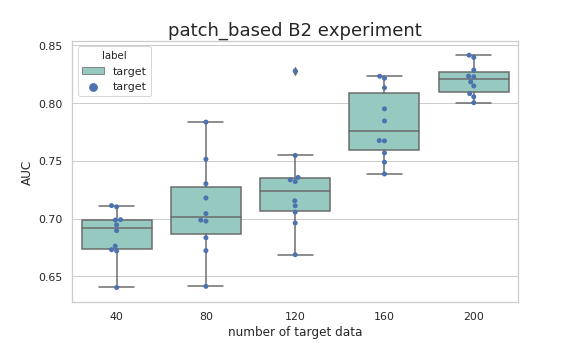
\includegraphics[width=\textwidth]{fig/B2_num_patch.png}
        \caption{\label{fig:parallel1} Patch-based AUC for B2 Experiment}
    \end{minipage}
    \hfil
\end{figure}
\begin{figure}[H]
    \hfil
    \begin{minipage}[t]{0.9\textwidth}
        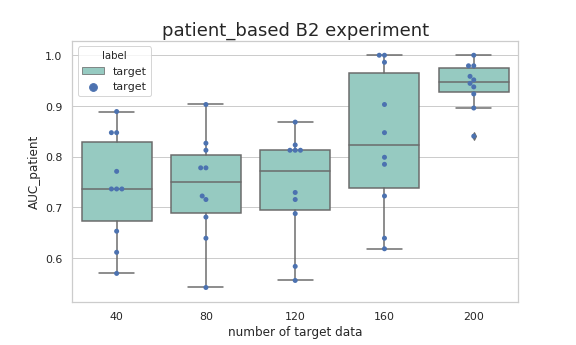
\includegraphics[width=\textwidth]{fig/B2_num_patient.png}
        \caption{\label{fig:parallel1} Patient-based AUC for B2 Experiment}
    \end{minipage}
    \hfil
\end{figure}

\subsection{Choose the Number of Fixed Layers in Fine-tuning Experiments (B3)}
This experiment is applied to choose the number of fixed layers. Fine-tuning is an efficient method to improve the AUC performance on target data. Therefore choosing the number of layers fixed is an important issue for further experiments.

Ten-folder cross-validation was performed to get 10 fine-tuning data models. Figure 4.5 and figure 4.6 show the patch-based and patient-based AUC performance of experiment B3, respectively. Two hundred target data is applied in this experiment. Models fixing no layers or models fixing the first three layers have the highest AUC. However, fixing the first three layers needs less calculation time, so I choose to fix the first three layers in fine-tuning and incremental learning experiments. 
\begin{figure}[H]
    \hfil
    \begin{minipage}[t]{0.9\textwidth}
        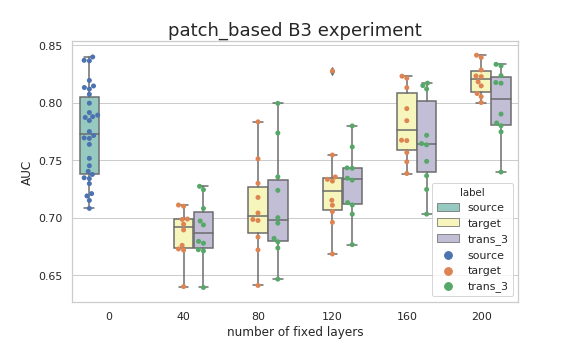
\includegraphics[width=\textwidth]{fig/B3_num_patch.png}
        \caption{\label{fig:parallel1}Patch-based AUC for B3 Experiment}
    \end{minipage}
    \hfil
\end{figure}
\begin{figure}[H]
    \hfil
    \begin{minipage}[t]{0.9\textwidth}
        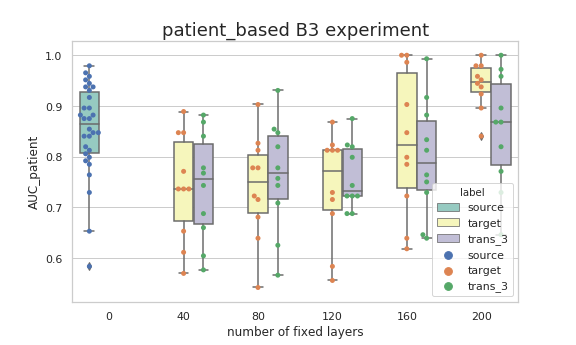
\includegraphics[width=\textwidth]{fig/B3_num_patient.png}
        \caption{\label{fig:parallel1} Patient-based AUC for B3 Experiment}
    \end{minipage}
    \hfil
\end{figure}

~\\
\section{Mixed Data Models}
\subsection{Mixed Data Models (M1)}
This experiment shows the simplest way to improve model AUC using source dataset. In this experiment, I mixed source dataset and target dataset and set this new dataset as the training set. 

Ten-folder cross-validation was performed to get 10 mixed data models. Figure 4.7 and figure 4.8 show the patch-based and patient-based AUC performance of experiment M1, respectively. 

In this experiment, the AUC increases as the number of target data increases. Although this experiment actually improves the AUC performance, it takes too much time on training since is the training set composed of both source and target dataset.

\begin{figure}[H]
    \hfil
    \begin{minipage}[t]{0.9\textwidth}
        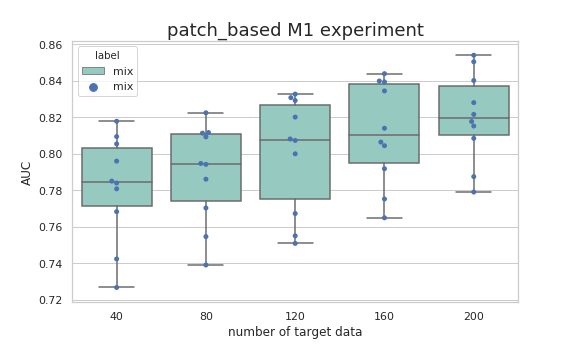
\includegraphics[width=\textwidth]{fig/M1_num_patch.png}
        \caption{\label{fig:parallel1}Patch-based AUC for M1 Experiment}
    \end{minipage}
    \hfil
\end{figure}
\begin{figure}[H]
    \hfil
    \begin{minipage}[t]{0.9\textwidth}
        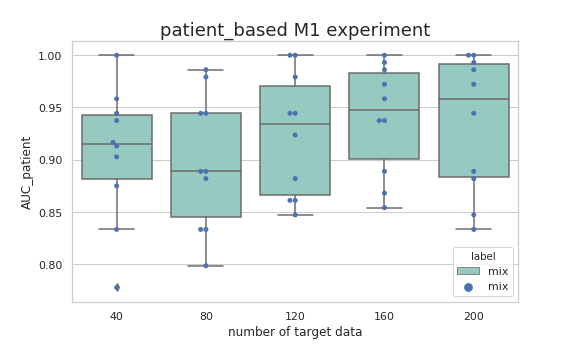
\includegraphics[width=\textwidth]{fig/M1_num_patient.png}
        \caption{\label{fig:parallel1}Patient-based AUC for M1 Experiment}
    \end{minipage}
    \hfil
\end{figure}
~\\
\section{Fine-Tuning Models}
\subsection{Fine-Tuning Models (F1)}
Fine-tuning, a kind of transfer learning method, is applied in this experiment to increase AUC of source data model (B1). The first three layers are fixed in this experiment based on the result of experiment B3.

Ten-folder cross-validation was performed to get 10 mixed data models. Figure 4.9 and figure 4.10 show the patch-based and patient-based AUC performance of experiment F1, respectively. 

In this experiment, the AUC increases as the number of target data increases. It takes less time on training compared to experiment M1 since is the training set (for fine tuning) composed of only target dataset.

\begin{figure}[H]
    \hfil
    \begin{minipage}[t]{0.9\textwidth}
        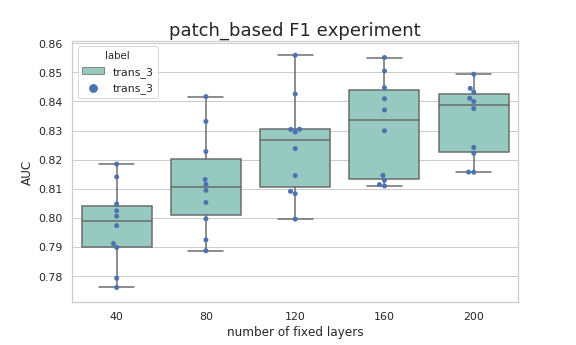
\includegraphics[width=\textwidth]{fig/F1_num_patch.png}
        \caption{\label{fig:parallel1}Patch-based AUC for F1 Experiment}
    \end{minipage}
    \hfil
\end{figure}
\begin{figure}[H]
    \hfil
    \begin{minipage}[t]{0.9\textwidth}
        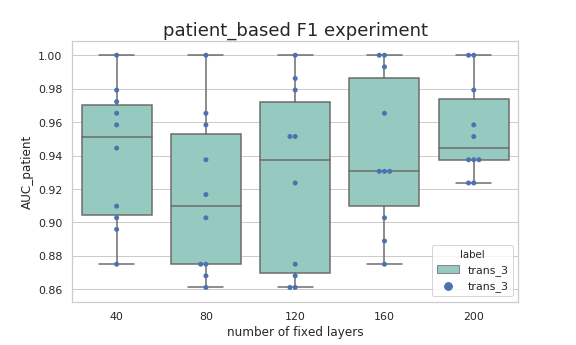
\includegraphics[width=\textwidth]{fig/F1_num_patient.png}
        \caption{\label{fig:parallel1} Patient-based AUC for F1 Experiment}
    \end{minipage}
    \hfil
\end{figure}
~\\
\section{Incremental Fine-Tuning Models}
In this part, I test the algorithm in thesis \cite{zhou2017fine} on pancreatic images to validate the algorithm performance. 
\subsection{Fine-tuning Using Selected/Random Target Data (S1/R1)}
This experiment is applied to observe the AUC performance and validate if the selection method AIFT works compared to random selection. Forty patient data is selected in each selection step. Since the difference among two selection method is highly empathized in the experiment, we use 200 epochs to run each selection steps to make sure that the training process won't stop too early. 

Ten-folder cross-validation was performed twice to get 20 mixed data models since the AUC results are not clear enough.
Figure 4.11, figure 4.12, figure 4.13 and figure 4.14 show the patch-based or patient-based AUC performance of experiment F1. 

In this experiment, the AUC increases as the number of target data increases. The AUC increase heavily compared to normal fine-tuning model, but increase slowly after the first selection step.

\begin{figure}[H]
    \hfil
    \begin{minipage}[t]{0.9\textwidth}
        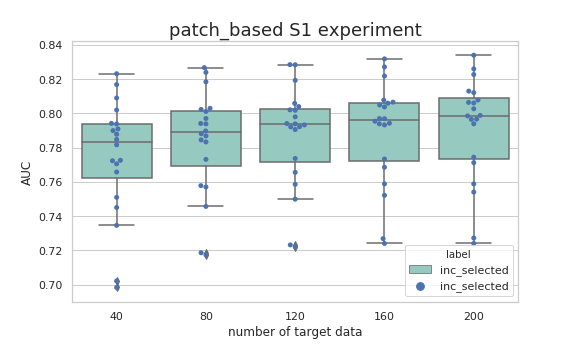
\includegraphics[width=\textwidth]{fig/S1_num_patch.png}
        \caption{\label{fig:parallel1}Patch-based AUC for S1 Experiment}
    \end{minipage}
    \hfil
\end{figure}
\begin{figure}[H]
    \hfil
    \begin{minipage}[t]{0.9\textwidth}
        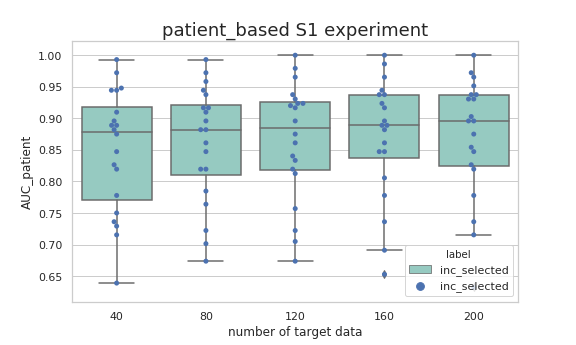
\includegraphics[width=\textwidth]{fig/S1_num_patient.png}
        \caption{\label{fig:parallel1}Patient-based AUC for S1 Experiment}
    \end{minipage}
    \hfil
\end{figure}
~\\
\begin{figure}[H]
    \hfil
    \begin{minipage}[t]{0.9\textwidth}
        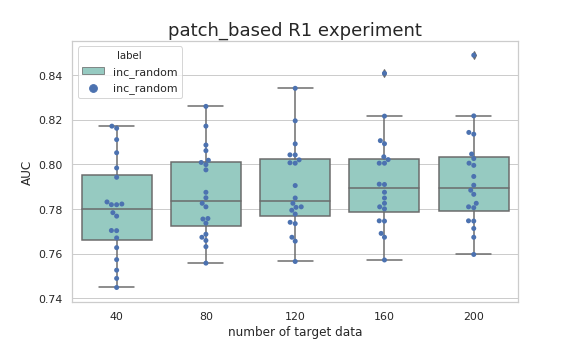
\includegraphics[width=\textwidth]{fig/R1_num_patch.png}
        \caption{\label{fig:parallel1}Patch-based AUC for R1 Experiment}
    \end{minipage}
    \hfil
\end{figure}
\begin{figure}[H]
    \hfil
    \begin{minipage}[t]{0.9\textwidth}
        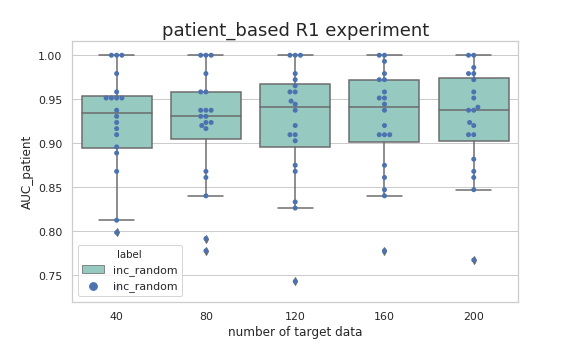
\includegraphics[width=\textwidth]{fig/R1_num_patient.png}
        \caption{\label{fig:parallel1}Patient-based AUC for R1 Experiment}
    \end{minipage}
    \hfil
\end{figure}
~\\
\subsection{Number of Target Data in each Selection Step (S2/R2)}

This experiment is applied to observe the AUC performance of incremental learning model with different selection steps. 

Ten-folder cross-validation was performed to get 10 mixed data models.
Figure 4.15, Figure 4.16, Figure 4.17 and figure 4.18 show the patch-based or patient-based AUC performance of experiment F1. 

In this experiment, the AUC increases as selection step increases. The AUC increase heavily when selection step is less than 60. The AUC performance is not stable in random selection experiments.

\begin{figure}[H]
    \hfil
    \begin{minipage}[t]{0.9\textwidth}
        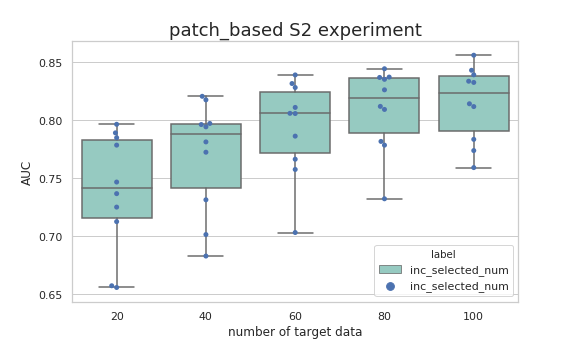
\includegraphics[width=\textwidth]{fig/S2_num_patch.png}
        \caption{\label{fig:parallel1}Patch-based AUC for S2 Experiment}
    \end{minipage}
    \hfil
\end{figure}
\begin{figure}[H]
    \hfil
    \begin{minipage}[t]{0.9\textwidth}
        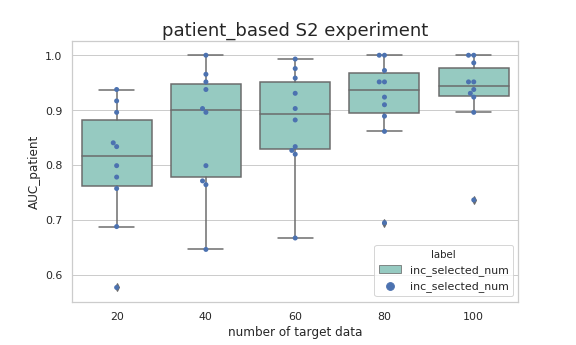
\includegraphics[width=\textwidth]{fig/S2_num_patient.png}
        \caption{\label{fig:parallel1}Patient-based AUC for S2 Experiment}
    \end{minipage}
    \hfil
\end{figure}
~\\
\begin{figure}[H]
    \hfil
    \begin{minipage}[t]{0.9\textwidth}
        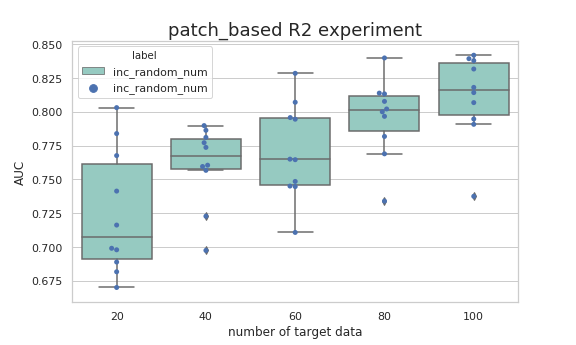
\includegraphics[width=\textwidth]{fig/R2_num_patch.png}
        \caption{\label{fig:parallel1} Patch-based AUC for R2 Experiment}
    \end{minipage}
    \hfil
\end{figure}
\begin{figure}[H]
    \hfil
    \begin{minipage}[t]{0.9\textwidth}
        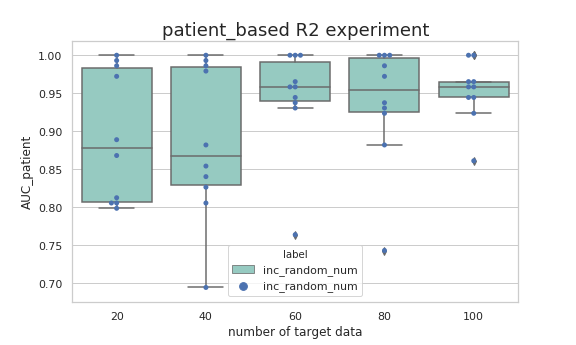
\includegraphics[width=\textwidth]{fig/R2_num_patient.png}
        \caption{\label{fig:parallel1}Patient-based AUC for R2 Experiment}
    \end{minipage}
    \hfil
\end{figure}
~\\

\subsection{Reduce the Epochs to Compare With Fine-tuning Experiments (S3/R3)}
This experiment is applied to observe the AUC performance of incremental learning model if both calculation waste are the same. Two hundred epochs is set for normal fine-tuning model (number of target data is 200), and 66 epochs is set for incremental learning (number of target data varies from 40 to 200). 

Ten-folder cross-validation was performed to get 10 mixed data models.
Figure 4.19, Figure 4.20, Figure 4.21 and figure 4.22 show the patch-based or patient-based AUC performance of experiment S3/R3. 

In this experiment, the AUC increases as target data increases.


\begin{figure}[H]
    \hfil
    \begin{minipage}[t]{0.9\textwidth}
        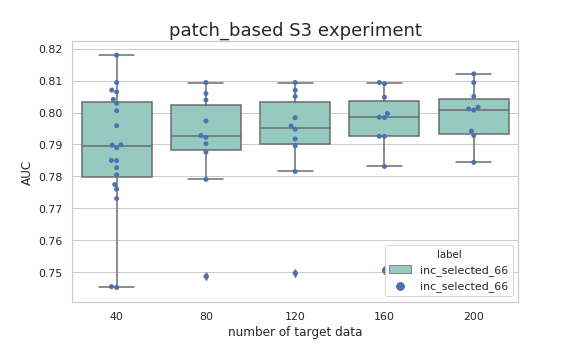
\includegraphics[width=\textwidth]{fig/S3_num_patch.png}
        \caption{\label{fig:parallel1}Patch-based AUC for S3 Experiment}
    \end{minipage}
    \hfil
\end{figure}
\begin{figure}[H]
    \hfil
    \begin{minipage}[t]{0.9\textwidth}
        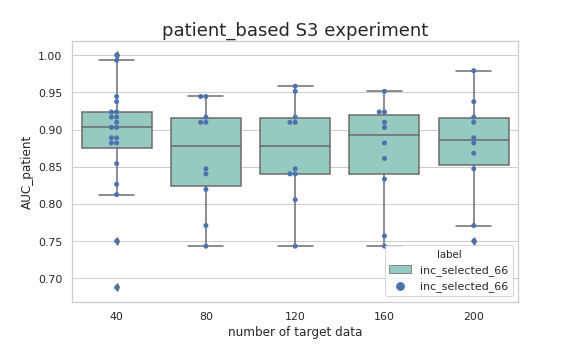
\includegraphics[width=\textwidth]{fig/S3_num_patient.png}
        \caption{\label{fig:parallel1}Patient-based AUC for S3 Experiment}
    \end{minipage}
    \hfil
\end{figure}
~\\
\begin{figure}[H]
    \hfil
    \begin{minipage}[t]{0.9\textwidth}
        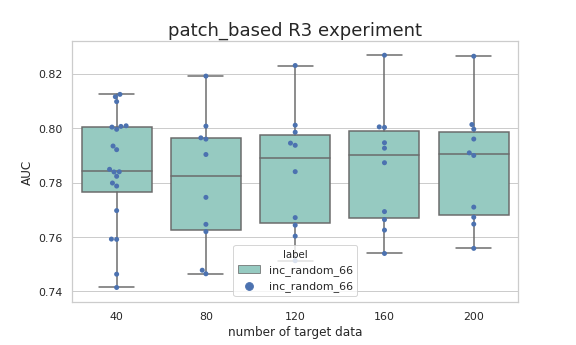
\includegraphics[width=\textwidth]{fig/R3_num_patch.png}
        \caption{\label{fig:parallel1}Patch-based AUC for R3 Experiment}
    \end{minipage}
    \hfil
\end{figure}
\begin{figure}[H]
    \hfil
    \begin{minipage}[t]{0.9\textwidth}
        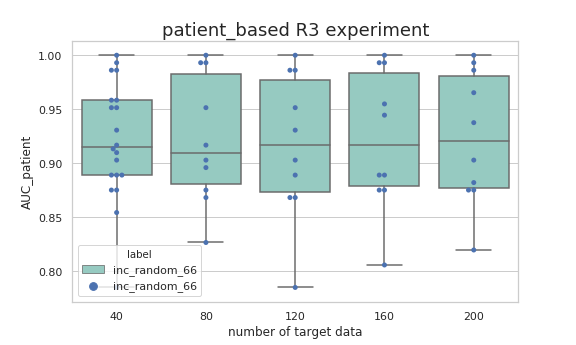
\includegraphics[width=\textwidth]{fig/R3_num_patient.png}
        \caption{\label{fig:parallel1}Patient-based AUC for R3 Experiment}
    \end{minipage}
    \hfil
\end{figure}
~\\


The sections below compares the experiments from section 3.1 to 3.4. 

\section{The AUC Performance of mixed Data Experiments}
I compared the AUC performance of source data model (B1), target data model (B2), and mixed data model (M1). The mixed data model highly improves AUC performance especially when the number of target data is small. It is a simple way to improve the performance by adding target data into training dataset. But the disadvantage is also clear. The calculation cost is huge since the number of training data is large compared with other methods.
 \\

\begin{figure}[H]
    \hfil
    \begin{minipage}[t]{0.9\textwidth}
        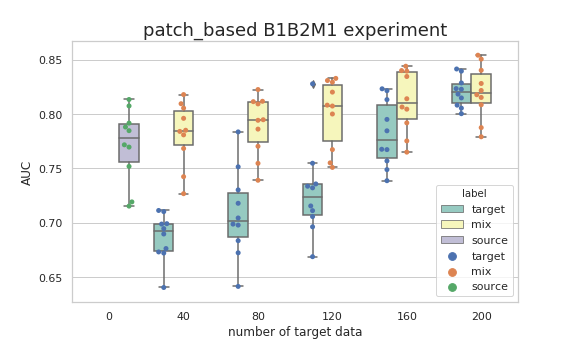
\includegraphics[width=\textwidth]{fig/B1B2M1_num_patch.png}
        \caption{\label{fig:parallel1}Patch-based AUC for B1B2M1 Experiment}
    \end{minipage}
    \hfil
\end{figure}
\begin{figure}[H]
    \hfil
    \begin{minipage}[t]{0.9\textwidth}
        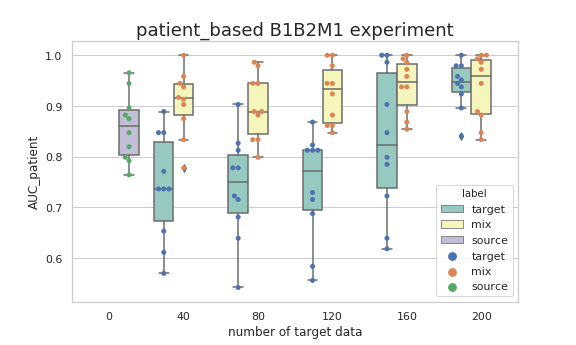
\includegraphics[width=\textwidth]{fig/B1B2M1_num_patient.png}
        \caption{\label{fig:parallel1}Patient-based AUC for B1B2M1 Experiment}
    \end{minipage}
    \hfil
\end{figure}

\section{The AUC Performance of Fine-Tuning Experiments}
I compared the AUC performance of source data model (B1), target data model (B2), and fine-tuning model (F1). The fine-tuning model highly improves AUC performance especially when the number of target data is small. It improves the disadvantage of mixed data model. The calculation speed is fast since it only need to train target data if we already have source data model. 
 \\

\begin{figure}[H]
    \hfil
    \begin{minipage}[t]{0.9\textwidth}
        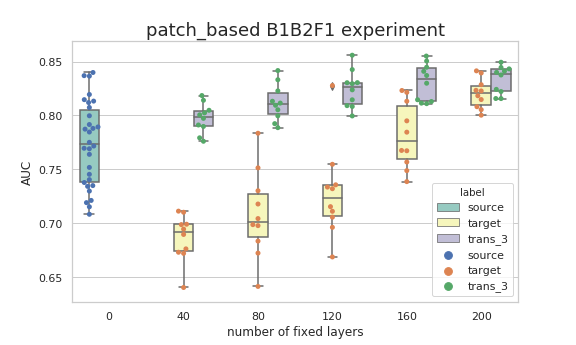
\includegraphics[width=\textwidth]{fig/B1B2F1_num_patch.png}
        \caption{\label{fig:parallel1}Patch-based AUC for B1B2F1 Experiment}
    \end{minipage}
    \hfil
\end{figure}
\begin{figure}[H]
    \hfil
    \begin{minipage}[t]{0.9\textwidth}
        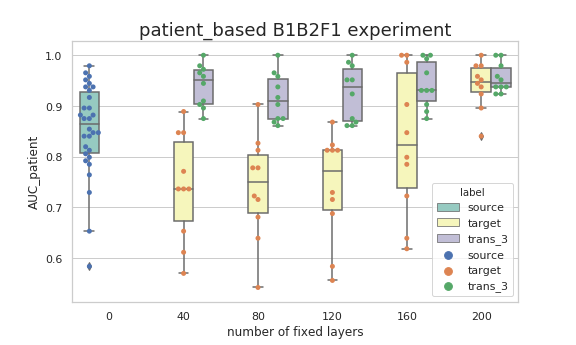
\includegraphics[width=\textwidth]{fig/B1B2F1_num_patient.png}
        \caption{\label{fig:parallel1}Patient-based AUC for B1B2F1 Experiment}
    \end{minipage}
    \hfil
\end{figure}


\section{Comparison of Mixed Data Experiments and Fine-Tuning Experiments}

I compared the AUC performance of source data model (B1), mixed data model (M1), and fine-tuning model (F1). mixed data model and fine-tuning model both improve the performance, but fine-tuning model performs better than mixed data model with lower calculation cost. Obviously fine-tuning method is a workable method to improve the AUC performance applied on target data. 
 \\

\begin{figure}[H]
    \hfil
    \begin{minipage}[t]{0.9\textwidth}
        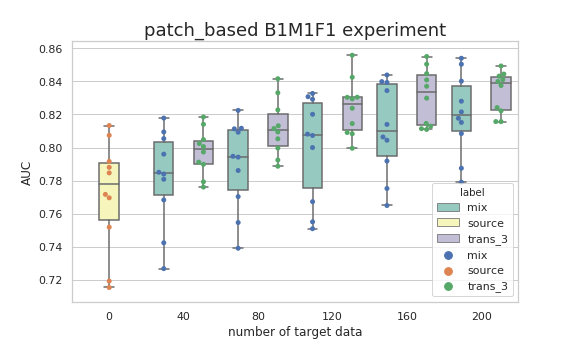
\includegraphics[width=\textwidth]{fig/B1M1F1_num_patch.png}
        \caption{\label{fig:parallel1} Patch-based AUC for B1M1F1 Experiment}
    \end{minipage}
    \hfil
\end{figure}
\begin{figure}[H]
    \hfil
    \begin{minipage}[t]{0.9\textwidth}
        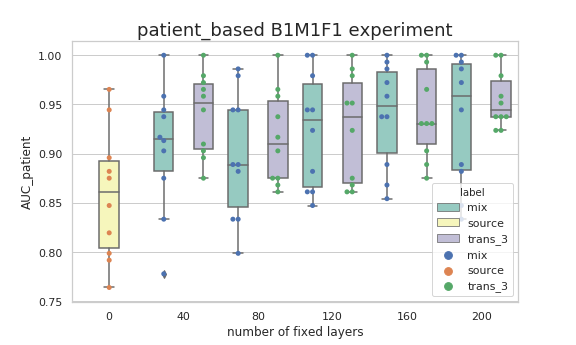
\includegraphics[width=\textwidth]{fig/B1M1F1_num_patient.png}
        \caption{\label{fig:parallel1} Patient-based AUC for B1M1F1 Experiment}
    \end{minipage}
    \hfil
\end{figure}
\section{Validation of Selection Method in incremental Learning}
incremental learning is a modified method of fine-tuning. We compared the result of different selection. The selection method of S1 experiment is AIFT method mentioned in thesis \cite{zhou2017fine} while R1 experiment use random selection instead of AIFT method. 
We observe that in patch-based result, the AUC performance of AIFT method is slightly better than random method but the patient-based result is not. There might be several reasons. First, the way we transfer the patch-based result into patient-based result may need to be modified. Second, the selected data can't improve the AUC performance of patient-based prediction. It needs further experiments to validate these two assumptions.  

\begin{figure}[H]
    \hfil
    \begin{minipage}[t]{0.9\textwidth}
        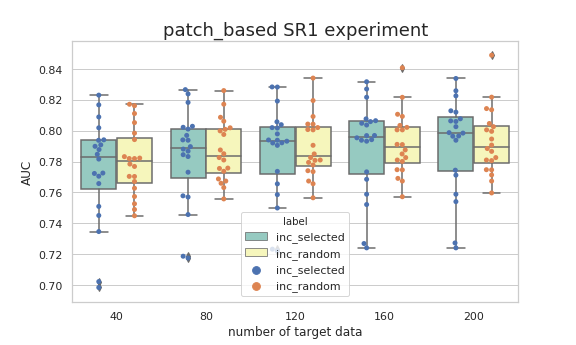
\includegraphics[width=\textwidth]{fig/SR1_num_patch.png}
        \caption{\label{fig:parallel1} Patch-based AUC for S1R1 Experiment}
    \end{minipage}
    \hfil
\end{figure}
\begin{figure}[H]
    \hfil
    \begin{minipage}[t]{0.9\textwidth}
        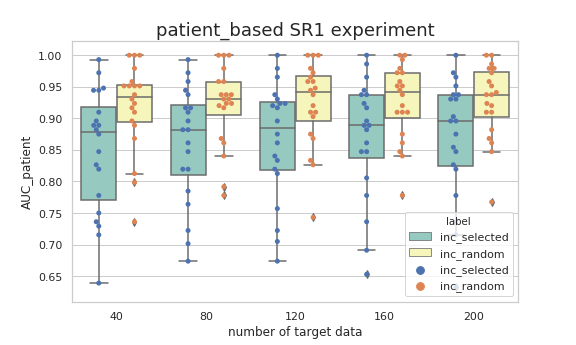
\includegraphics[width=\textwidth]{fig/SR1_num_patient.png}
        \caption{\label{fig:parallel1} Patient-based AUC for S1R1 Experiment}
    \end{minipage}
    \hfil
\end{figure}


\section{Comparison of Fine-Tuning Experiments and Incremental Learning Experiments}
I compared the AUC performance of source data model (B1), fine-tuning model (F1), and selected incremental learning model (S1). The selected incremental learning model can't provide obvious difference by selection method. Another problem is that the performance incremental learning stop early compared with fine-tuning. I drew the validation loss diagram and found that the loss almost didn't decrease after first 50 epochs. This algorithm may estimate too much on the first few data it selected and only find a local minimum in training process.

\begin{figure}[H]
    \hfil
    \begin{minipage}[t]{0.9\textwidth}
        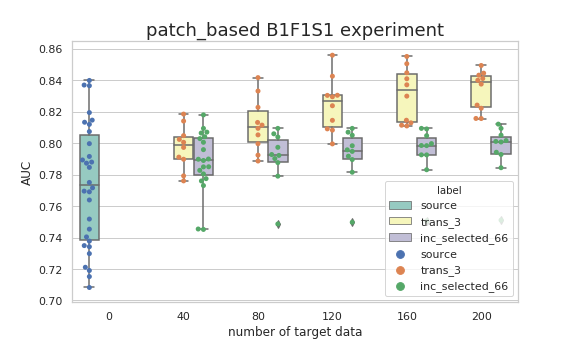
\includegraphics[width=\textwidth]{fig/B1F1S1_num_patch.png}
        \caption{\label{fig:parallel1}Patch-based AUC for B1F1S1 Experiment}
    \end{minipage}
    \hfil
\end{figure}
\begin{figure}[H]
    \hfil
    \begin{minipage}[t]{0.9\textwidth}
        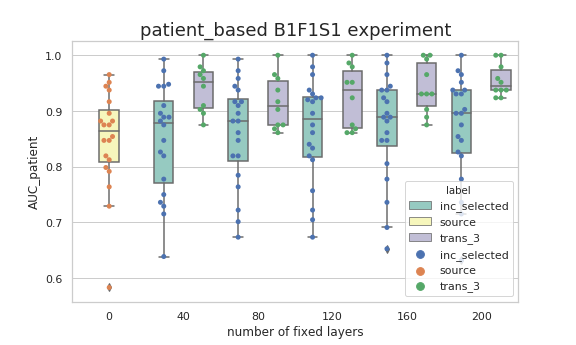
\includegraphics[width=\textwidth]{fig/B1F1S1_num_patient.png}
        \caption{\label{fig:parallel1}Patient-based AUC for B1F1S1 Experiment}
    \end{minipage}
    \hfil
\end{figure}
\begin{figure}[H]
    \hfil
    \begin{minipage}[t]{0.9\textwidth}
        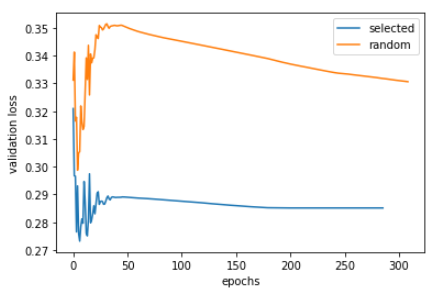
\includegraphics[width=\textwidth]{fig/loss.png}
        \caption{\label{fig:parallel1} Validation Loss of Selected/Random Incremental Learning}
    \end{minipage}
    \hfil
\end{figure}
\chapter{Discussion}
\section{Limitations} 
((Study limitations, including potential bias, statistical uncertainty, and generalizability)) \\
Since the target data is composed of two dataset: MSD dataset and TCIA dataset, the distribution of two datasets might be different, so the model performance may decrease because of the reason. Also, since the number of data is not large enough, the outliers shows up in cross validation experiments. 

\section{Implications for practice*}
((Implications for practice, including the intended use and/or clinical role)) \\

\section{Future Work?}
We can try different fine-tuning details of AIFT method. It's possible to increase the performance on target data. 

\chapter{Other*}
\section{Information}

\subsection{Registration number and name of registry}
\subsection{Where the full study protocol can be accessed}
\subsection{Sources of funding and other support; role of funders}




\printindex


\bibliographystyle{abbrv}
\bibliography{mybib}
\addcontentsline{toc}{chapter}{Bibliography}
%\appendix
%\begin{appendices}
% 	\chapter{Proof for example}
% 	\section{title}
% 	Here we consider the case of $q= 12289 $, $k=3$.
% 	The input $U,V$ satisfies the following condition.
% 	\begin{center}
% 		$V = V_0+V_1 \cdot 2^{12} + V_2 \cdot 2^{24}$ and
% 		$U = U_0 + U_1 \cdot 2^{12} $\\
% 	\end{center}
	
	
% 	where 
% 	$0 \leq V_0 < 2^{12}$,
% 	$0 \leq V_1 < 2^{12}$,
% 	$0 \leq V_2 < 2^{6}$,
% 	$0 \leq U_0 < 2^{12}$, and 
% 	$0 \leq U_1 < 2^{4}$ 
% 	%
% 	\begin{center}
% 		$A = \texttt{K-RED}(U)  = 3 U_0 - U_1$ and
% 		$B = \texttt{K-RED2x}(V)  = 9 V_0 - 3 V_1 + V_2$ 
% 	\end{center}

	
	
%\end{appendices}



\end{document}